\documentclass[letterpaper,10pt,twocolumn]{article}

\usepackage[backend=bibtex,style=numeric,citestyle=numeric]{biblatex}
\bibliography{report}


\usepackage{fullpage}

\usepackage{amsmath}
\usepackage{amssymb}
\usepackage{amsthm}
\usepackage{enumerate}
\usepackage{listings}
\usepackage{algpseudocode}
\usepackage{changepage}  %%for adjustwidth macro
\usepackage{verbatim}
\usepackage{float}
\usepackage{graphicx}
\usepackage{epstopdf}
\usepackage{url}

\title{COMP 7150 --- Data Science Project Report}
\author{
    Hicks, Eric\\
    \texttt{elhicks@memphis.edu}
    \and
    Kelly, Craig\\
    \texttt{cnkelly@memphis.edu}
}

\begin{document}

% Force pdflatex to properly use letter as page size (instead
% of defaulting to A4)
\special{papersize=8.5in,11in}
\setlength{\pdfpageheight}{\paperheight}
\setlength{\pdfpagewidth}{\paperwidth}

\maketitle

\abstract{
Te Steam video game store is a source for interesting data about video game
use, including consumer behavior and industry sales. A single, usable data
set is not available from the Steam Store, but there are available API's.
These API's and other public resources were used to create a single, clean,
flat data set for public exploration. Some initial hypotheses about what should
be seen in the data were made and tested as part of this project. All code and
data has been publicly available for use by others.
}

%%%%%%%%%%%%%%%%%%%%%%%%%%%%%%%%%%%%%%%%%%%%%%%%%%%%%%%%%%%%%%%%%%%%%%%%%%%%
%%%%%%%%%%%%%%%%%%%%%%%%%%%%%%%%%%%%%%%%%%%%%%%%%%%%%%%%%%%%%%%%%%%%%%%%%%%%

\section{Introduction}

In this paper, the path and results of the authors' dissection of the Steam
platform will be detailed. The reason Steam was chosen for this project, was
due to its large acceptance in the PC space. Steam is a company that sells
PC, Mac, and Linux games for download over the Internet. With weekly sales,
daily releases, a managed library, and no computer limit on games, it is the
largest digital distributor of games and the most widely used. Additionally,
Steam stores metrics on over a 100 million users on nearly 10,000 games,
making it a perfect example of a feature rich dataset. However, as Steam has
no saved repository of data publicly available, one was created for this
project, hereby called the Steam dataset. \cite{steam}


%%%%%%%%%%%%%%%%%%%%%%%%%%%%%%%%%%%%%%%%%%%%%%%%%%%%%%%%%%%%%%%%%%%%%%%%%%%%
%%%%%%%%%%%%%%%%%%%%%%%%%%%%%%%%%%%%%%%%%%%%%%%%%%%%%%%%%%%%%%%%%%%%%%%%%%%%

\section{Steam Dataset}

This dataset and analysis project was inspired by the SteamDB project
\cite{steamdb}. SteamDB does not provide data for download, and does not
provide an API. SteamDB uses the SteamKit2 library \cite{steamkit} for
acessing the Steam API \cite{steamdb-faq}. This does not appear to unusual;
for instance the site Rhekua \cite{rhekua} makes no data available either.

Unlike SteamDB and other services, one service will data available for
download was found. The service ``Steam Spy'' makes their data available via
API, and that API includes a full download \cite{steamspy}. The Steam Spy data
is gathered via web scraping performed on a random sample of Steam user pages
using a technique originally described by Ars Technica
\cite{steamspy-about,steamgauge}. The technique depends on the format of Steam
user ID's, the URL for Steam user pages, and the data shown on a user's
profile page. This dataset was used to include owner and player counts in our
final data set of video game features (please see section \ref{data-grab}).

\subsection{Acquisition}

\label{data-grab}

SteamKit2 is designed for the entire API made available by Steam
\cite{steamkit}, much of which requires a developer/partner agreement with
Steam \cite{steam-dev}. The authors chose to use SteamKit2 as a starting point,
but to write their own, slim data acquisition library.

The entire process of acquiring, cleaning, and formatting is automated in a
Makefile in the ``data'' subdirectory of the public GitHub repository for this
project \cite{our-github}. This process is shown visually in figure
\ref{fig:data-flow}.

\begin{figure}[H]
    \label{fig:data-flow}
    \caption{Data flow used to produce the final data set}
    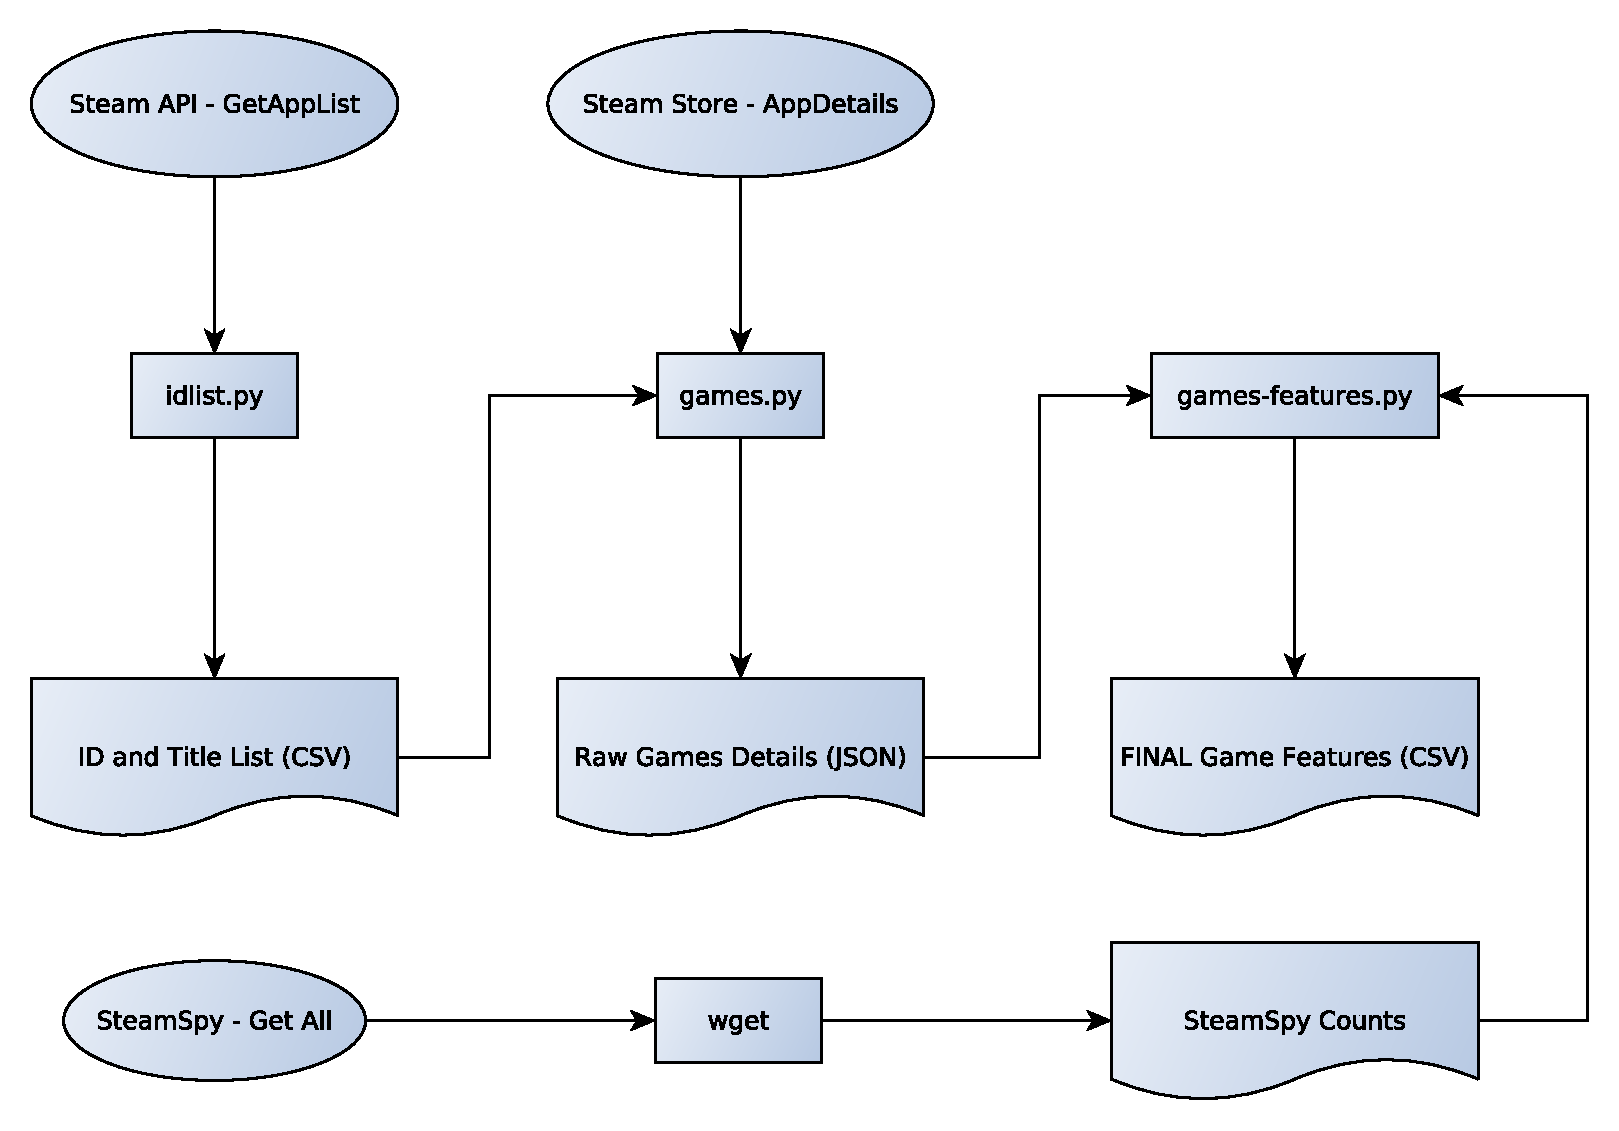
\includegraphics[width=0.45\textwidth,keepaspectratio]{data-flow}
\end{figure}

The official Steam API has a few endpoints that are usable without an official
API key. One of them provides a list of applications ID's and titles. These
``application'' ID's actually refer anything made available in the Steam
store, including movies, video trailers, downloadable content, etc. This list
is saved as a two column CSV named ``idlist.csv''.

Once an ID list is obtained, the bulk of the data retrieval process can begin.
The script ``games.py'' was written to get the details of each ID one at a
time from the Steam Store API. Each response is saved in it's original JSON
form as a line in the file ``games.json''.

At one time bulk retrieval was allowed, but that is no longer the case so one
request must be made per ID. In addition, the Steam Store throttles requests
to around 200 queries per five minutes according to online sources. This limit
is honored by pausing for five minutes and ten seconds every 150 requests.
Even so, occasionally the Steam Store would stop accepting requests from the
IP address used by the script. As a result, the script was updated to handle
repeated execution. When running, all ID's already in the output file are
skipped.

New games are constantly added to Steam. In addition, the detail data
retrieved is constantly changing as users play games, vendors alter prices,
etc. In an attempt to get the most and best data, the retry logic above was
used to check and retrieve all current data from Steam on two occasions after
the initial data gathering was complete. Because the code is publicly
available, this same process could be used in the future to keep the data
``fresh''.

An additional file of details per Steam ID is downloaded from Steam Spy using
the ``wget'' command line tool. Around 13 numeric fields are provide for Steam
ID's in a single, huge JSON record.

The final stage of execution is the script ``game-features.py'', which creates
the final data set in ``game-features.csv'' using the data files already
created. This stage is described in section \ref{data-clean}.


\subsection{Cleaning and Formatting}

\label{data-clean}

TODO: reduced to 78 fields
TODO: explain field removal

\subsection{Metacritic}

While many of the data dimensions are self-explanatory, Metacritic might
require some explanation. Metacritic provides a rating service for video
games, movies, television shows, and music \cite{metacritic}. The Metacritic
score is a proprietary weighted average of various professional critics and
publications, scaled from 1 to 100 \cite{metacritic-score}. It is one of the
most frequently used metrics for video game quality \cite{metacritic-vgdominant}.


\subsection{Caveats}

The process used could not capture all data dimensions used by Steam. Some are
not recorded and others can only be accessed by an administrator account. The
number of owners for each game could not be acquired, but has been estimated
using an outside site \cite{steamspy}. Recommendations were collected as a
total of reviews and as two separate values for positive and negative reviews.
The sentiment of the reviews that Steam displays was also not able to be
captured. Steam doesn't store historical price data, so sale history and
price trends can not be analyzed from the data. These limitations did not stop
the authors from gaining interesting insight from the data.


%%%%%%%%%%%%%%%%%%%%%%%%%%%%%%%%%%%%%%%%%%%%%%%%%%%%%%%%%%%%%%%%%%%%%%%%%%%%
%%%%%%%%%%%%%%%%%%%%%%%%%%%%%%%%%%%%%%%%%%%%%%%%%%%%%%%%%%%%%%%%%%%%%%%%%%%%

\section{Predictions}

As both authors were familiar with Steam before the start of the project, they
made some predictions of what would be found in the data:

TODO: more predictions

\begin{enumerate}
    \item SteamOS games available on Steam would be a perfect match to Linux
    games available.

    \item The most recommended and the highest rated genre is action.

    \item That Metacritic scores are an inverse bell curve when sorted by
    recommendation, i.e. lower and higher scoring games would have more
    recommendations that games with a middle score.

    \item That free games get more reviews per game and have lower ratings than
    paid games.
\end{enumerate}


%%%%%%%%%%%%%%%%%%%%%%%%%%%%%%%%%%%%%%%%%%%%%%%%%%%%%%%%%%%%%%%%%%%%%%%%%%%%
%%%%%%%%%%%%%%%%%%%%%%%%%%%%%%%%%%%%%%%%%%%%%%%%%%%%%%%%%%%%%%%%%%%%%%%%%%%%

\section{Testing}

Both authors ran different models on the data independent of each other to
cover the most ground. Every feature pair was plotted as a scatter plot to
gain a basic understanding of feature relations alongside reading through the
raw data. From here other options were tried.


%%%%%%%%%%%%%%%%%%%%%%%%%%%%%%%%%%%%%%%%%%%%%%%%%%%%%%%%%%%%%%%%%%%%%%%%%%%%
%%%%%%%%%%%%%%%%%%%%%%%%%%%%%%%%%%%%%%%%%%%%%%%%%%%%%%%%%%%%%%%%%%%%%%%%%%%%

\section{Results}

The authors found results corresponding to all predictions. Some other interesting
results were found as a result of exploratory analysis.

TOOD: craig's analysis

\subsection{SteamOS and Linux}

As a sanity check, the authors insure that a simple prediction was verifiable
by the dataset. By definition, all Steam games available on the Linux platform
must also be on the SteamOS platform because SteamOS is only way to run a Steam
game on Linux. The data verified this ``prediction''.

TODO: figure for SteamOS and Linux

\subsection{Free vs Non-Free Games}

Free games do get more recommendations than paid games (see figure
\ref{fig:freevnon-ratings}). However, they are also lower rated lower than paid
games (see figure \ref{fig:freevnon-metacritic}). In fact, ``free to play'' as a
genre received the most feedback via recommendations (see figure
\ref{fig:genre-ratings}), but had the lowest rating scores (see figure
\ref{fig:genre-metacritic}). As a result, we conclude that free games tend to
have negative reviews; in fact, the plurality of reviews for free games might
well be negative. (TODO: last sentence in ``Future Work''.)

\begin{figure}[H]
    \label{fig:freevnon-ratings}
    \caption{Count of recommendations from users on Free vs Non-Free games}
    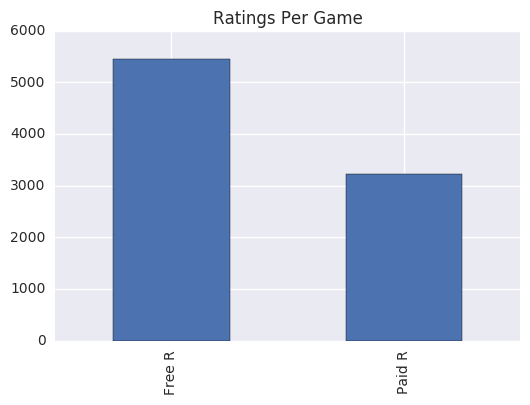
\includegraphics[width=0.45\textwidth,keepaspectratio]{freevnon-ratings-bar}
\end{figure}

\begin{figure}[H]
    \label{fig:freevnon-metacritic}
    \caption{Metacritic mean score on Free vs Non-Free games}
    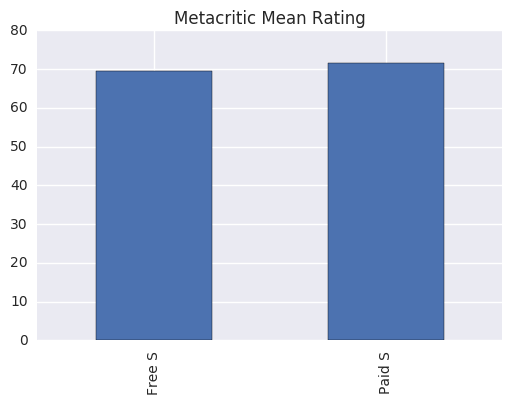
\includegraphics[width=0.45\textwidth,keepaspectratio]{freevnon-metacritic-bar}
\end{figure}


\subsection{Genre}

The most recommended genre was free to play and not action. The least
recommended genre was non-game software (see figure \ref{fig:genre-ratings}).
The highest scoring genre was sports instead of action. The lowest
scoring genre was free to play (see figure \ref{fig:genre-metacritic}).

\begin{figure}[H]
    \label{fig:genre-ratings}
    \caption{Count of recommendations from users by genre}
    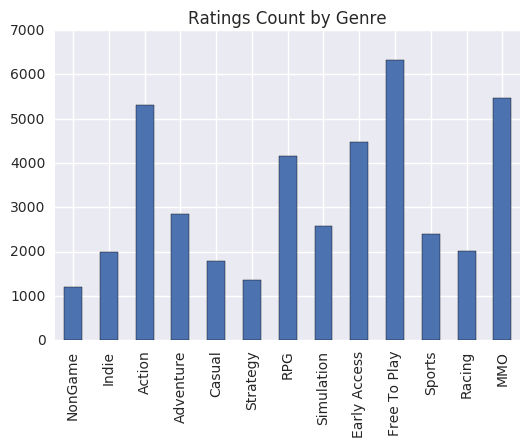
\includegraphics[width=0.45\textwidth,keepaspectratio]{genre-ratings-bar}
\end{figure}

\begin{figure}[H]
    \label{fig:genre-metacritic}
    \caption{Metacritic mean score by genre}
    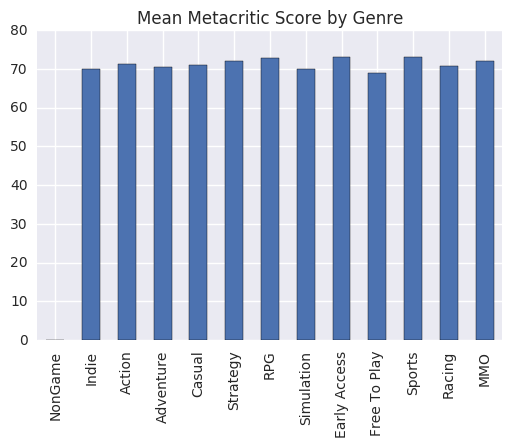
\includegraphics[width=0.45\textwidth,keepaspectratio]{genre-metacritic-bar}
\end{figure}

\subsection{Recommendations, Ratings, and Price}

Although not part of the original prediction, some relationships (or lack
thereof) were noticed. Pricing compared to Metacritic scores is mostly
uniform. The gaps for certain prices are almost entirely due to Steam's
pricing structure. Pricing compared to user recommendations is also nearly
uniform. There is a small increase in recommendations for cheaper games, but
it is not significant. Please see figures
\ref{fig:metacritic-recommendations},
\ref{fig:metacritic-price}, and
\ref{fig:price-recommendations}.

\begin{figure}[H]
    \label{fig:metacritic-recommendations}
    \caption{Relationship of Count of User Recommendations to Metacritic Score}
    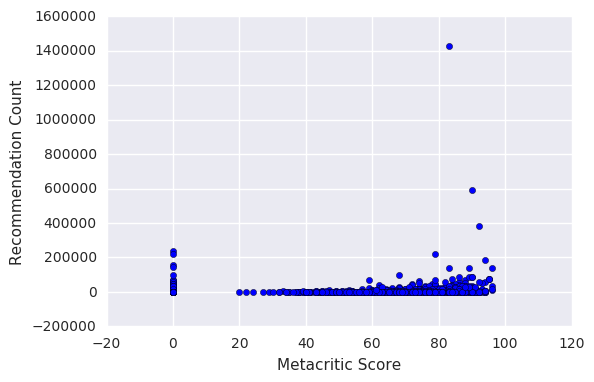
\includegraphics[width=0.45\textwidth,keepaspectratio]{metacritic-recommendations-scatter}
\end{figure}

\begin{figure}[H]
    \label{fig:metacritic-price}
    \caption{Relationship of Metacritic Score to Initial Price}
    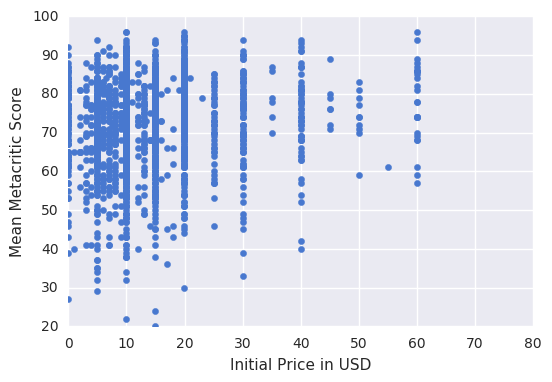
\includegraphics[width=0.45\textwidth,keepaspectratio]{price-metacritic-scatter}
\end{figure}

\begin{figure}[H]
    \label{fig:price-recommendations}
    \caption{Relationship of Initial Price to Count of User Recommendations}
    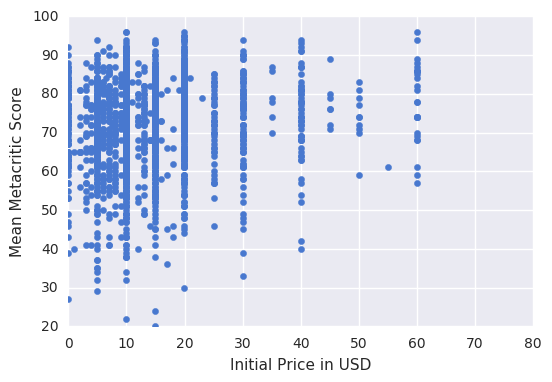
\includegraphics[width=0.45\textwidth,keepaspectratio]{price-metacritic-scatter}
\end{figure}


%%%%%%%%%%%%%%%%%%%%%%%%%%%%%%%%%%%%%%%%%%%%%%%%%%%%%%%%%%%%%%%%%%%%%%%%%%%%
%%%%%%%%%%%%%%%%%%%%%%%%%%%%%%%%%%%%%%%%%%%%%%%%%%%%%%%%%%%%%%%%%%%%%%%%%%%%

\section{Future Work}

Given a larger timespan to collect data and more sophisticated web crawlers,
more data come be pulled from Steam. This would allow for most, if not all of
the caveats mentioned before to be removed. With historical data, price
trends for games of different genres could be predicted along with the time
frames for price drops. A divided recommendation statistic could be used to
determine if certain genres get more positive reviews than others, as well as
show a correlation (or lack thereof) between Metacritic scores and positive
recommendations.

%%%%%%%%%%%%%%%%%%%%%%%%%%%%%%%%%%%%%%%%%%%%%%%%%%%%%%%%%%%%%%%%%%%%%%%%%%%%
%%%%%%%%%%%%%%%%%%%%%%%%%%%%%%%%%%%%%%%%%%%%%%%%%%%%%%%%%%%%%%%%%%%%%%%%%%%%

\section{Conclusion}

After finding a suitable platform to mine data from, the authors acquired raw
data from Steam. This data was cleaned, formatted, and processed to find
several interesting results. While all of the authors' predictions were not
proven in testing, the ones that were wrong proved to be the most surprising.

TODO: more text

TODO: appendix with field listing? or just a link to the repo?

%%%%%%%%%%%%%%%%%%%%%%%%%%%%%%%%%%%%%%%%%%%%%%%%%%%%%%%%%%%%%%%%%%%%%%%%%%%%%
% Bibliography
%%%%%%%%%%%%%%%%%%%%%%%%%%%%%%%%%%%%%%%%%%%%%%%%%%%%%%%%%%%%%%%%%%%%%%%%%%%%%

\nocite{*}                                 % ensure we show the entire bib
\printbibliography

%%%%%%%%%%%%%%%%%%%%%%%%%%%%%%%%%%%%%%%%%%%%%%%%%%%%%%%%%%%%%%%%%%%%%%%%%%%%
%%%%%%%%%%%%%%%%%%%%%%%%%%%%%%%%%%%%%%%%%%%%%%%%%%%%%%%%%%%%%%%%%%%%%%%%%%%%

\end{document}
